
%(BEGIN_QUESTION)
% Copyright 2005, Tony R. Kuphaldt, released under the Creative Commons Attribution License (v 1.0)
% This means you may do almost anything with this work of mine, so long as you give me proper credit

Define what ``derivative'' means when applied to the graph of a function.  For instance, examine this graph:

$$\includegraphics[width=15.5cm]{i01509x01.eps}$$

Label all the points where the derivative of the function ($dy \over dx$) is positive, where it is negative, and where it is equal to zero.

\vskip 20pt \vbox{\hrule \hbox{\strut \vrule{} {\bf Suggestions for Socratic discussion} \vrule} \hrule}

\begin{itemize}
\item{} Articulate a set of simple rules for determining whether a point on a curve has a derivative that is positive, negative, or zero.  These rules should be simple enough for a child to comprehend and apply!
\item{} Sometimes the slope of a curved function at any given point is graphically shown by something called a {\it tangent line}.  Research what a ``tangent line'' is, and then draw tangent lines on this function to demonstrate the slope at some specified points.
\end{itemize}

\underbar{file i01509}
%(END_QUESTION)





%(BEGIN_ANSWER)

The graphical interpretation of ``derivative'' means the {\it slope} of the function at any given point.

$$\includegraphics[width=15.5cm]{i01509x02.eps}$$

%(END_ANSWER)





%(BEGIN_NOTES)

Usually students find the concept of the derivative easiest to understand in graphical form: being the {\it slope} of the graph.  This is true whether or not the independent variable is time (an important point given that most ``intuitive'' examples of the derivative are time-based!).

%INDEX% Mathematics, calculus: derivative (defined in a graphical sense)

%(END_NOTES)


